\graphicspath{{Chapitre_2/Images/}}
\chapter{Notions of thermodynamics}\label{C2}
%%%%%%%%%%%%%%%%%%%%%%%%%%%%%%%%%%%
%%%%%                         %%%%%
%%%%% Introduction chapitre 2 %%%%%
%%%%%                         %%%%%
%%%%%%%%%%%%%%%%%%%%%%%%%%%%%%%%%%%
\quad\, The principle and uses of the Brayton cycle have been discussed in the introduction. As explained, this concept has been applied for many usages, including electricity production and aircraft propulsion which are the most common and known applications. It has been exposed that from the invention proposed by George Brayton in the end of the 19th century, the technology did really evolve.

Indeed, while the Brayton cycle engine first appears as a  piston engine where the compression, combustion and expansion occur in the same enclosure. Nowadays the process is shared between at least three components (namely the compressor, the turbine and the combustion chamber).

However, the key notions to understand how theses components behave have not been introduced yet. This problematic will be covered by this chapter, which will introduce step-by-step those notions.
\section{Open/closed system}\label{sect:C2_Sys}
\quad\,  The thermodynamic is a science that ''studies the exchange of energy between a system and its environment or surroundings'' \cite{thermoApp_1}.
The system is defined as being the area of the space selected for the study. Between the system and the environment lies the boundary. This boundary can either be real or fictitious and can be static or mobile.

When the system is characterized, it has to be defined if it is an open or a closed system.

On one hand, closed systems do not exchange matter with the environment. Those systems are characterized by a control mass well delimited in the space of study. Therefore, only heat or work can be transferred from the system to the surroundings.

On the other hand, the open systems are ones where an arbitrary control volume well demarcated in the space is studied. In contrast to closed systems, open systems not only exchange work and heat with the environment, but also matter. Typical examples are the combustion chamber, heat exchanger, turbomachines, piping,...

\section{State Functions}\label{sect:C2_State}
\quad\, Let considered a system as defined in the previous section. The state functions are defined as ''a property of the system that only depends on its current state.” These functions are independent of the past of the system and describe the equilibrium state of the system.

When the state functions can be measured (directly or indirectly), these are called state variables. For example, the pressure $p$, the temperature $T$ or the volume $\mathrm{V}$ is state variables.

In this work, the units used for the state and function variables follow the international system (SI) of units \cite{Nist}. 
\subsection{Pressure}
\quad\, The pressure unit is the Pascal (Pa). 1 Pa corresponds to 1 N/m$^2$, where 1 N (kg$\cdot$m/s$^2$) is the required force to increase each second by 1m/s the velocity of a body of 1kg.

The pressure is also often expressed in bar, unit corresponding to 1e5 Pa.
\subsection{Temperature}
\quad\, The temperature unit is the Kelvin (K). 273.15\degree K corresponds to 0\degree C, temperature at which pure water starts freezing.
\subsection{Volume}
\quad\, The volume unit is the meter cube (m$^3$).
\section{Ideal gas equation}
\quad\, It can be shown that the equilibrium state of a system can be described by those three variables. Also, among $p$,  $T$ and $\mathrm{V}$, only two of them are independent. 

This means that a state relation defined as \textbf{F}($p$, $T$, $\mathrm{V}$)= 0.

For the ideal gas, the most well known state relation is the relation of perfect gases defined in (\ref{eq:C2_GP}).

\begin{align}
\setstretch{1}
p\cdot \mathrm{V} &= m\cdot\frac{R}{MM}\cdot T\nonumber\\
p\cdot \mathrm{v} &= r\cdot T\label{eq:C2_GP}    
\end{align}
Where \textit{m} is the quantity of matter (kg), $R=8.314$ J/mole$\cdot$K is the universal gas constant, $\mathrm{v}$ the specific volume (m$^3$/kg) and $MM$ is the molar mass (kg/mole\footnote{Where one mole corresponds to $\sim 6\cdot 10^{23}$ elementary entities (atoms, molecules,...)}) of the system. 

The density $\rho$ of the gas is given as being one over the specific volume $\mathrm{v}$.
\section{Energy}\label{sect:C2_Ener}
\quad\, In the subsection \ref{sect:C2_Sys}, the notion of energy has been mentioned without characterizing it beforehand. From the first principle of the thermodynamic, it is stated that the energy cannot be created nor destroyed. Therefore, it can only be converted, meaning that the energy exists into multiple forms (thermal, mechanical, electrical,...)\cite{thermoApp_2}. 

The unit of the energy is the Joule (J), and the sum of all the energies in a system is called the total energy $E$. 1 Joule corresponds to the work required to move a body over 1 meter using a force of 1 N.

The energy is a state variable. This means that this quantity allows characterizing the state of the system. When considering the energy, its absolute value is not something that is defined. Instead, the energy is always computed as compared with a reference point.

Thus, considering the variation of the total energy from a state \textbf{1} to a state \textbf{2}, it is obtained that the total energy variation is equal to the sum of the variation of the internal, kinetic and potential energy $U$, $KE$ and $PE$ (respectively). The internal energy is defined as being the  sum of all the ''microscopic'' energy within the system (J).  

The definition of the total energy variation is given in the relation (\ref{eq:C2_E}).

\begin{equation}
\setstretch{1}
    \Delta E = \Delta U + \Delta KE + \Delta PE \label{eq:C2_E}
\end{equation}
\begin{align*}
\setstretch{1}
    \text{with } \Delta U  &= U_2 - U_1 =  m\cdot(u_2 - u_1) \text{: Variation of the internal energy}\\
                 \Delta KE &= \frac{1}{2}m\cdot(v^2_2 - v^2_1)\text{: Variation of the kinetic energy}\\
                 \Delta PE &= m\cdot \text{g}\cdot(z_2 - z_1)\text{: Variation of the potential energy}
\end{align*} 
Where $\text{g}=9.81$ m/s$^2$ is the acceleration on a body induced by the gravity, $z$ is the altitude of the system position (m), $v$ is the velocity of the fluid (m/s) and $u$ is the specific internal energy.


As said in the subsection \ref{sect:C2_Sys}, any system will exchange energy with the surroundings as heat and work. The heat is defined as ''the form of energy which is exchanged between the system and its environment when there is a gradient of temperature between these two entities''. 

As the heat is always referred as a flux between two bodies, the phenomenon is called heat transfer. The heat transfer can be realized by
\begin{itemize}
\setstretch{1}
    \item Conduction: Heat transfer through a non-flowing material due to the interaction of ''molecular scale energy carriers within the material''\cite{GregoryNellis2015}
    \item Convection: More complex conduction when considering a flowing fluid.
    \item Radiation: The heat is transferred as electromagnetic waves.
\end{itemize}
The heat transfer is denoted $Q$. A system that does not exchange heat with the surroundings is called \textbf{adiabatic}.

Aside the heat transfer, the system can also exchange energy by producing a work. The work $W$ is ''the form of energy exchanged associated to a force applied over a certain distance''. 

The work is exchanged if the force applied to the system creates a displacement of its boundary. The power is defined as the work per unit of time and is expressed in Watt (or W).

Both heat and work are called ''path functions'' because they are associated with the evolution of a system and not to the state of this system. Thus, these are not thermodynamic variables (like the temperature or the pressure).
\subsection{Energy balance}
\quad\, It has been previously mentioned several mechanisms to exchange energy from the system to its environment. Aside from the heat transfer and the work transfer, the energy can also be exchanged using mass transfer. 

Indeed, if the system is open, the mass entering and exiting the system will convey energy. To recall the first principle of the thermodynamic, the energy cannot be created or destroyed. 

Based on the statement, the energy balance of the system is given by the following generic formulation (\ref{eq:C2_EB}).
\begin{equation}
\setstretch{1}
    E_{in} - E_{out} = (Q_{in} - Q_{out}) + (W_{in} - W_{out}) + (E_{mass,in} - E_{mass,out}) = \Delta E_{system} \label{eq:C2_EB}
\end{equation}
With $E_{mass}$ the energy conveys by the mass entering/exiting the system.

It is possible to write a temporal formulation (\ref{eq:C2_PB}) of the energy balance named \textbf{power balance}.  
\begin{equation}
\setstretch{1}
    \dot{E}_{in} - \dot{E}_{out} = (\dot{Q}_{in} - \dot{Q}_{out}) + (\dot{W}_{in} - \dot{W}_{out}) + (\dot{E}_{mass,in} - \dot{E}_{mass,out}) = \frac{dE_{system}}{dt} \label{eq:C2_PB}
\end{equation}
Where $\frac{dE_{system}}{dt}=0$ when considering a system for which the variation of energy does not vary in the time.
\subsection{Energy conservation efficiency}
\quad\, When the system is transferring or converting energy, it is often interesting to quantify the quality of this transfer/conversion. The efficiency is defined to provide this quantification, and its definition is the
$\frac{\text{Desired ouptut}}{\text{Required input}}$. 

For example, a water electric heater with the efficiency of 90\% is a system such that 90\% of the electrical energy consumed is converted in thermal energy.  
Considering the combustion of fuel, the combustion efficiency is defined as the ratio
$$ \frac{\dot{Q}}{\dot{m}_{fuel}\cdot CV_{fuel}}$$
Where $\dot{m}_{fuel}$  and $HCV_{fuel}$ is the mass flow and the heating calorific value of the fuel injected into the combustion chamber.

\section{Phases}
\quad\ When a system is considered, the transformations that the system will see are usually applied on a fluid or a solid material. These elements are characterized by its level internal of energy and the surrounding conditions.

The phase of an element is defined based on the arrangement of the molecules constituting the elements. There exists three different type of phases:

\begin{itemize}
    \setstretch{1}
    \item Gas: The spacing between the molecules is large and the molecules are disordered. Each molecules are free to move within the gas in every direction.
    \item Liquid: There is an internal order within the liquid. The displacement of the molecules is limited to the translation and the rotation. The distance between each molecules is smaller than for the gas.
    \item Solid: The order is perfect. The molecules can only vibrate around their respective anchor point, and the distance between each molecules is a little bit smaller than for the liquid.
\end{itemize}

The three phases are illustrated in the Figures \ref{fig:C2_gas}, \ref{fig:C2_liq} and  \ref{fig:C2_sol}.

\begin{figure}[h]
     \centering
     \begin{subfigure}[b]{0.3\textwidth}
         \centering
         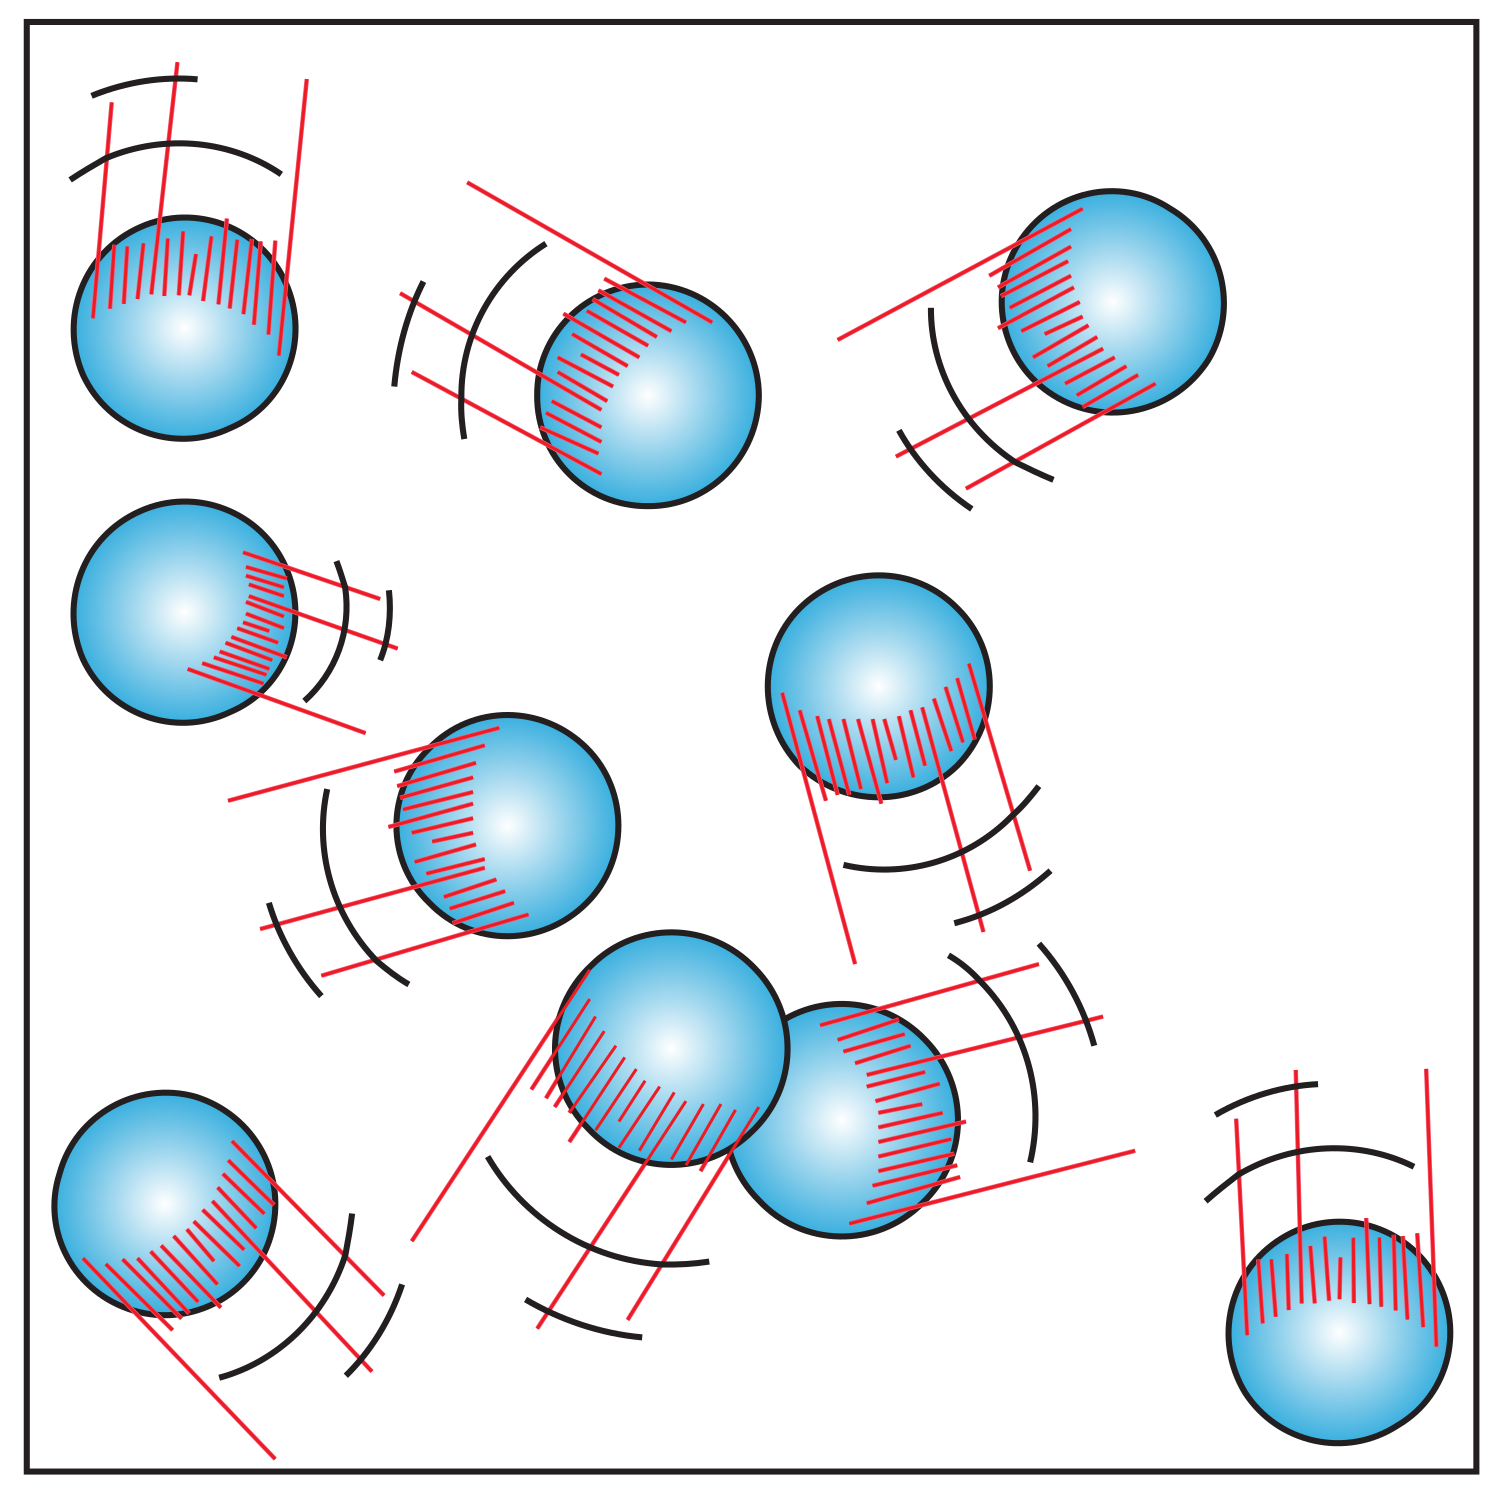
\includegraphics[width=\textwidth]{Chapitre_2/Images/gas.png}
         \caption{Gas.}
         \label{fig:C2_gas}
     \end{subfigure}
     \begin{subfigure}[b]{0.3\textwidth}
         \centering
         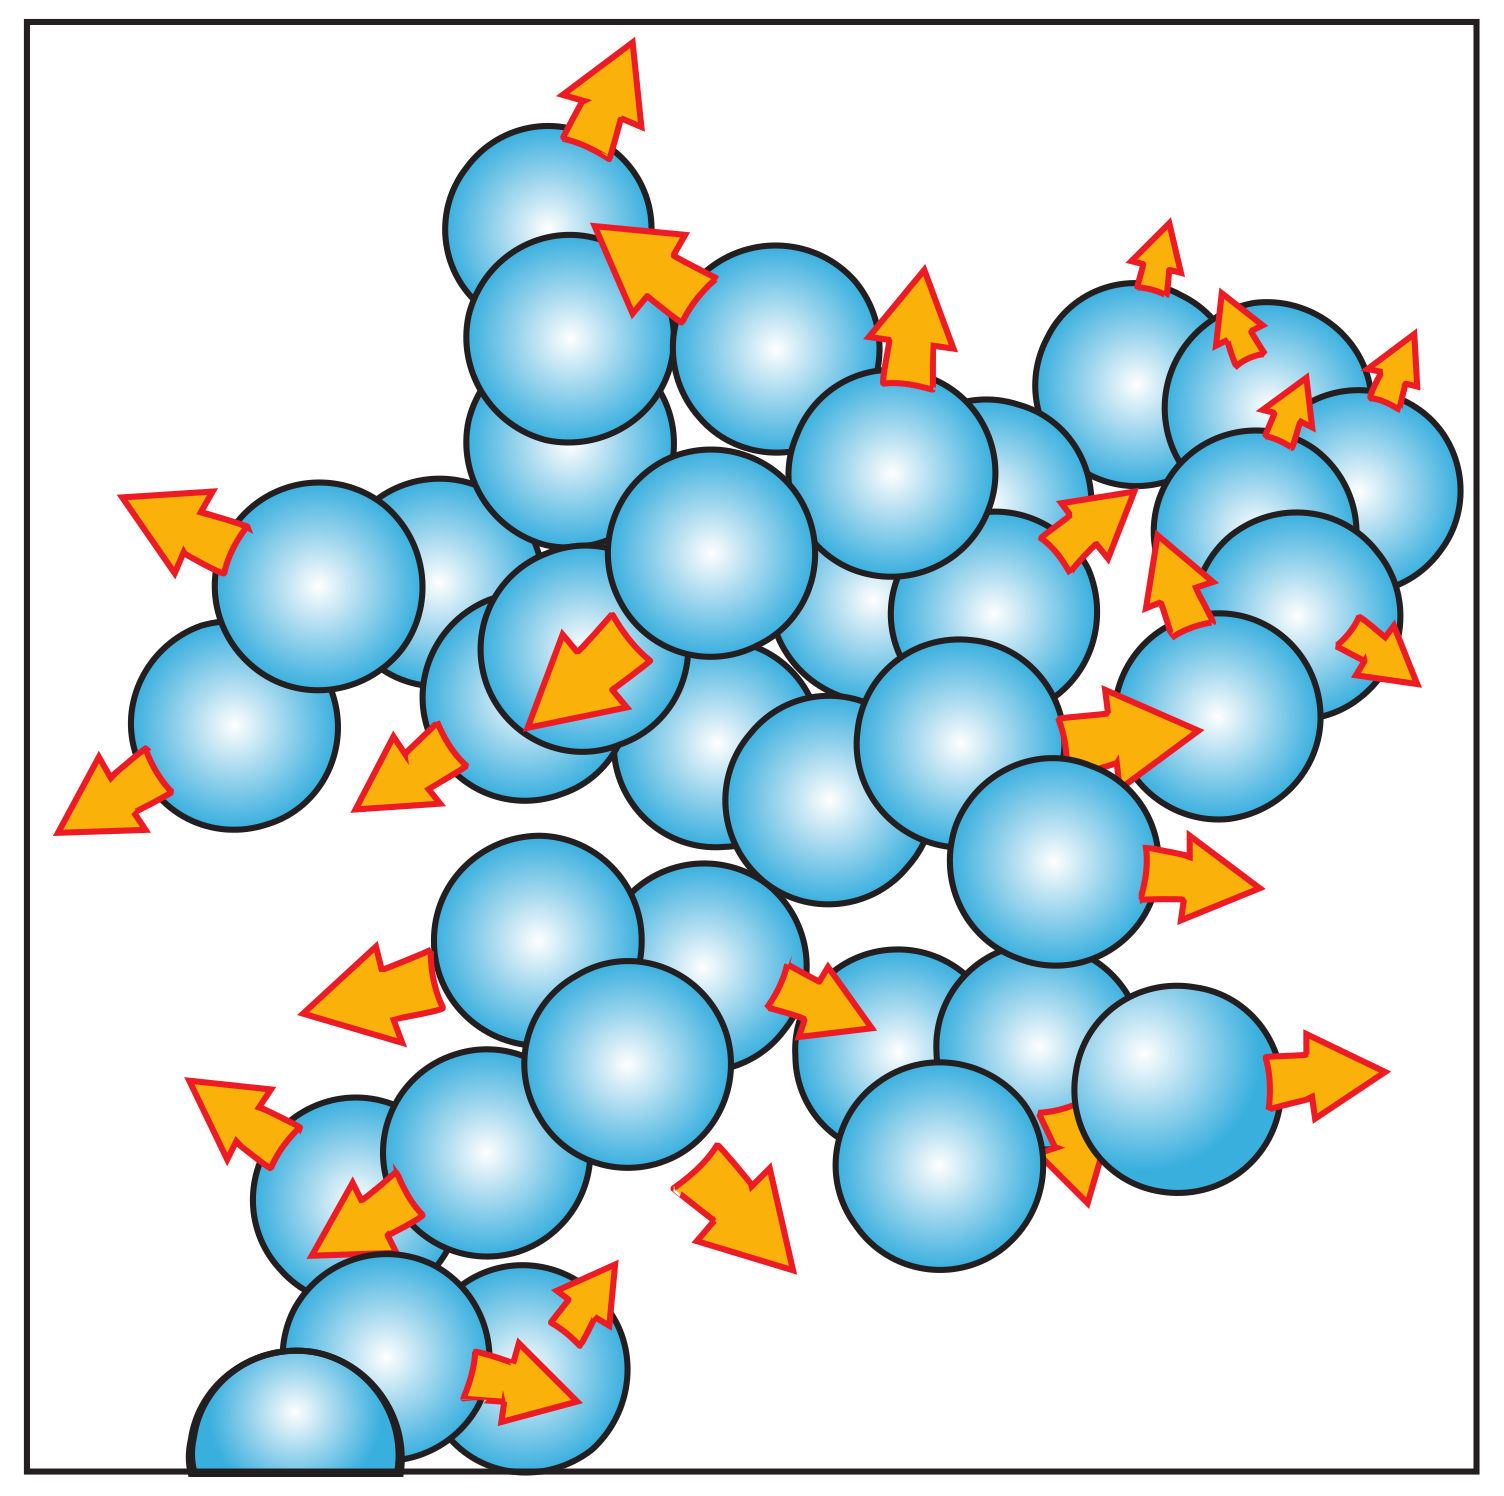
\includegraphics[width=\textwidth]{Chapitre_2/Images/liquid.png}
         \caption{Liquid.}
         \label{fig:C2_liq}
     \end{subfigure}
     \begin{subfigure}[b]{0.3\textwidth}
         \centering
         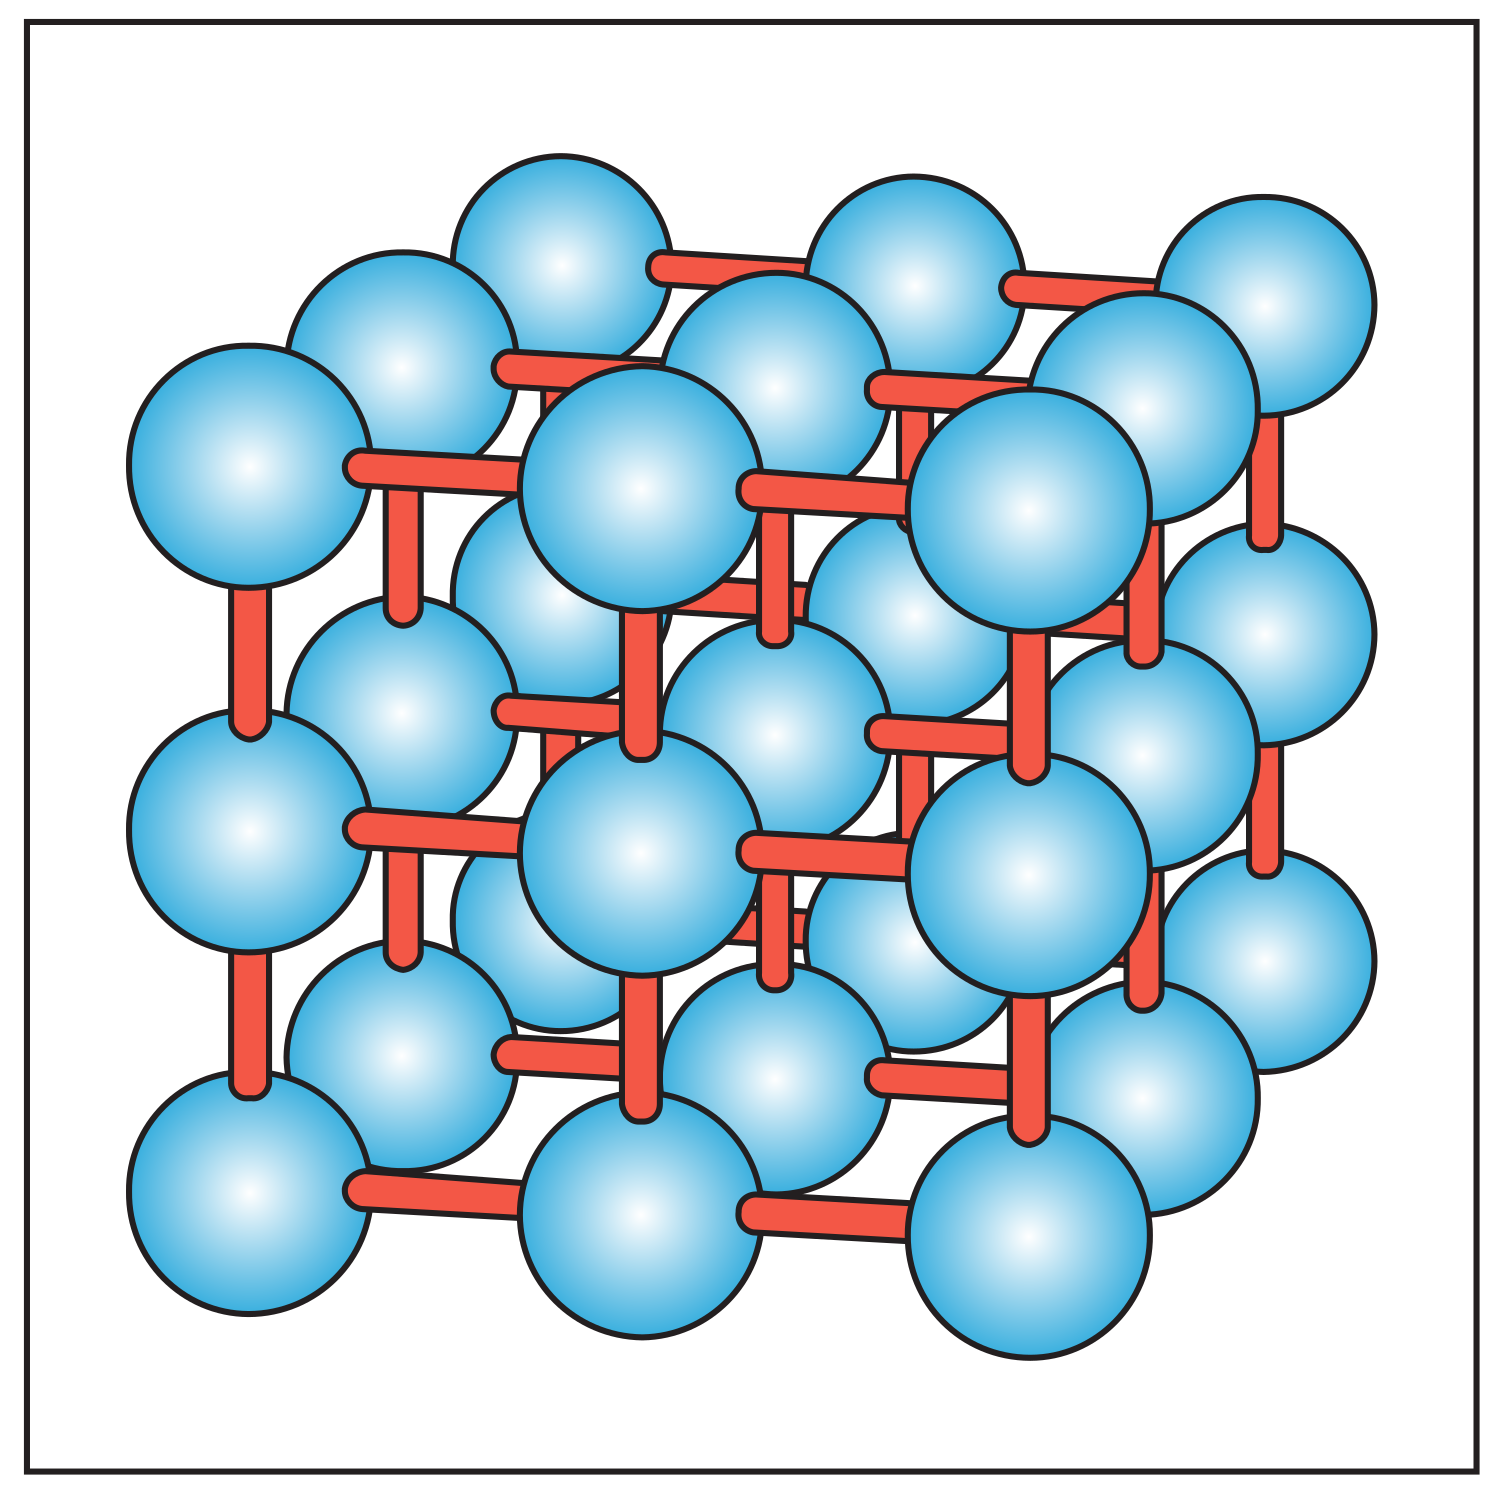
\includegraphics[width=\textwidth]{Chapitre_2/Images/solid.png}
         \caption{Solid.}
         \label{fig:C2_sol}
     \end{subfigure}
        \caption{Arrangement of the molecules depending the phases\cite{Boles2006}.}
        \label{fig:C2_phase}
\end{figure}

The phase of a given is determined by its level of energy and the surrounding conditions. When there is a transition from one phase to the other, the two phases are coexisting during the transition.
